\begin{frame}{Quản lý Hạ tầng dưới dạng mã}
\begin{figure}[H]
\centering
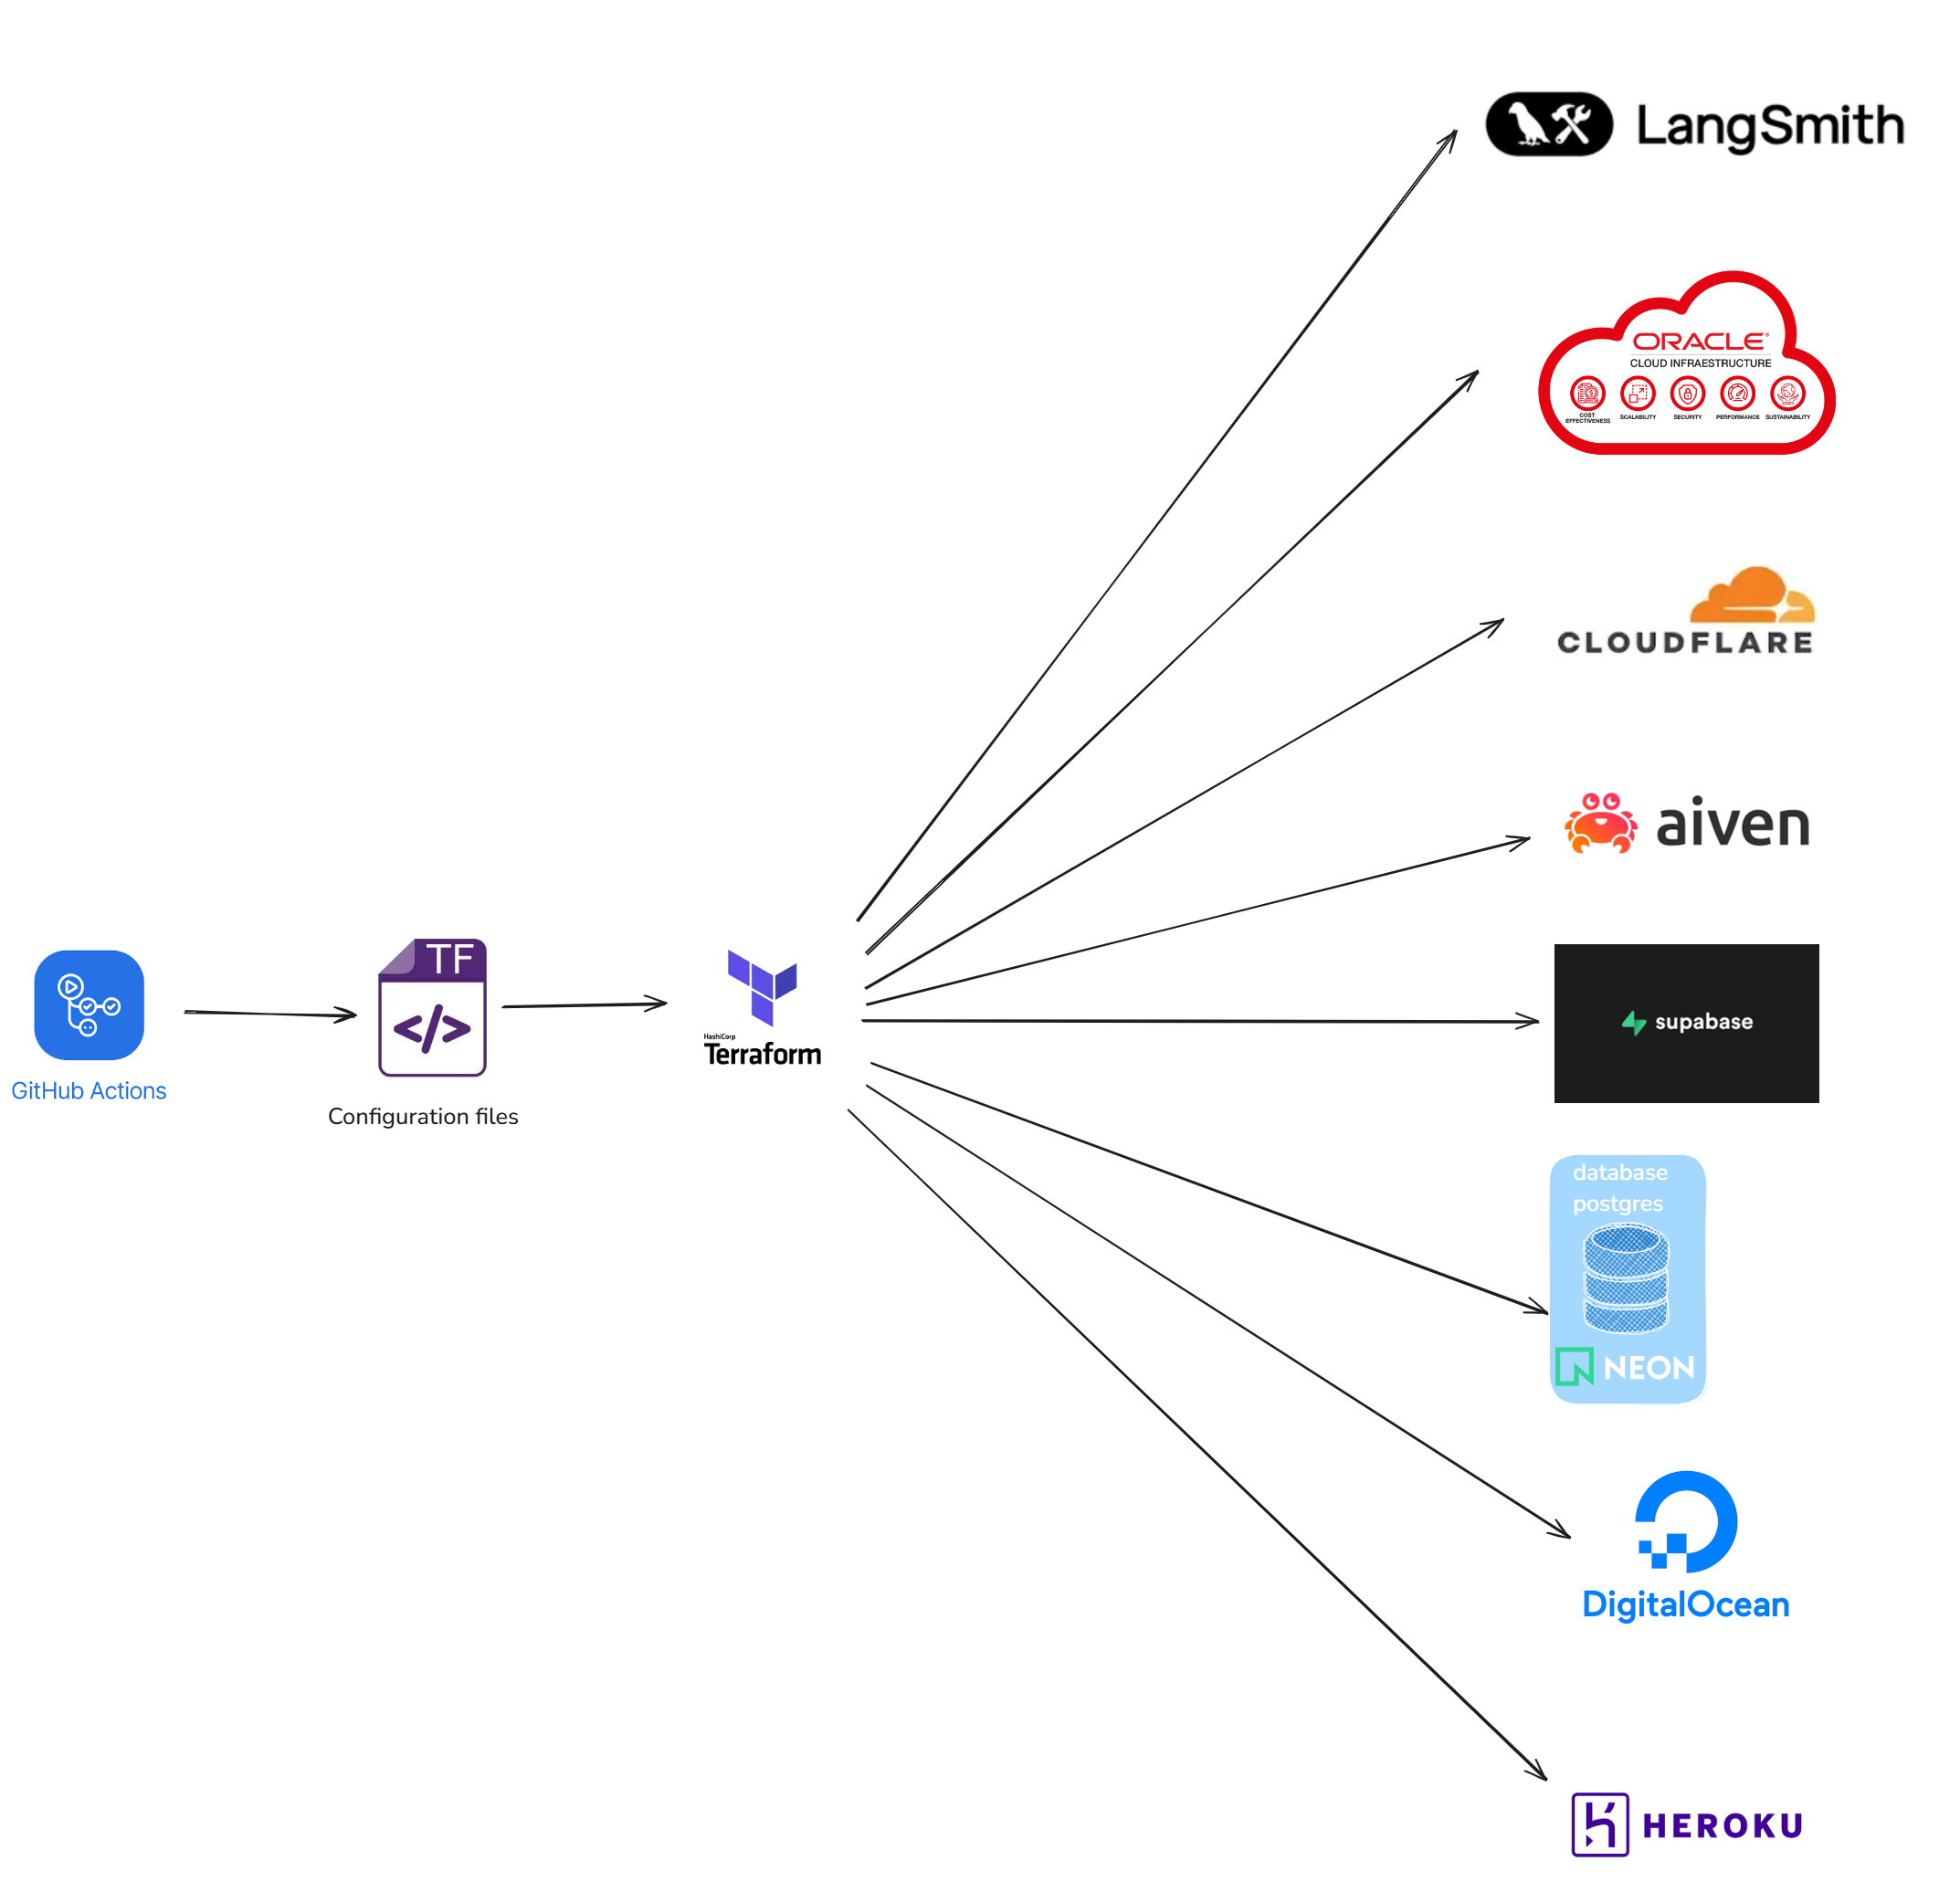
\includegraphics[height=0.7\textheight,width=0.9\textwidth,keepaspectratio]{pictures/infrastructure-as-code-IaC-terraform.excalidraw.png}
\caption{Sơ đồ tổng quan quản lý hạ tầng bằng Terraform trong dự án}
\end{figure}

\note{
Để quản lý hạ tầng một cách nhất quán và tự động, dự án sử dụng Terraform dưới dạng Infrastructure as Code (IaC).
Terraform tự động khởi tạo và cấu hình các tài nguyên bên thứ ba như: Supabase (Auth), LangSmith (giám sát RAG), Cloudflare (DNS và R2 Storage), Neon (PostgreSQL cho các vi dịch vụ), DigitalOcean (Crawl DB) và Heroku (Payment Service). Trạng thái hạ tầng được lưu trữ tập trung trên Terraform Cloud.
}
\end{frame}
